% !TeX spellcheck = en_US
\section{Existing Model Repositories}
\label{sec:background:modelrepo}
\todo{give some numbers from most}
Over the time modeling became one of the major methods in Computational and Systems Biology \citep{Finkelstein2004}. Thus more and more data in terms of models were produced and grow more complex \citep{Henkel2010}. As a result a number of projects require the reuse and recomposition of models, which prove to be difficult, if there is no central database available \citep{Waltemath2013}.
Out of this need, multiple projects started to collect, curate, and distribute models, to improve overall reuseability.
The two major model repositories, which I choose to focus on are, on one hand the \emph{BioModels Database}\footnote{\url{https://www.ebi.ac.uk/biomodels-main/}} \citep{Li2010}, focusing on \sbml encoded models and on the other hand the \emph{Physiome Model Repository}\footnote{\url{http://models.cellml.org/cellml}} (PMR2) \citep{Yu2011}, which is mainly providing \cellml encoded models.

However, these existing repositories provide a rich set of information about the model itself. It is now important to focus on associated information: integrating additional information, as simulation experiments descriptions (SED), result information, and publication and author references, will increase the reuseability of the models. \citep{Waltemath2013,Henkel2012}.


\begin{comment}
\begin{itemize}
	\item use/citep mostly introduction from \citep{Waltemath2013}
	\item maybe also citep \citep{Lysenko2016}?
\end{itemize}
\end{comment}

\section{Using graph databases to store \sysbio models}
\label{sec:backgroung:graph-db}
\todo{simplify this paragraph}
\sysbio models often encode simulation networks, which can easily be represented as graphs. These networks tend to be widely inhomogeneous, what proves a representation in a table based relational database to be inefficient and difficult, hence those databases are made to store highly structured information, e.g. numerical data. As a result the operations for combining information from different relations (joins) are expensive. On the other hand queries for traversing through the networks of models are essential for generating assumptions and basic information mining.
Further, data often needs to be converted to comply with the database schema, which implies changes, when new features are introduced to a model format. Moreover representing multiple standards results in a redundant schema, which makes it even harder to interlink this data. \citep{Lysenko2016}

In conclusion relational databases are less efficient in storing standard encoded models together with links to other data sources (e.g. ontologies), because there is no common schema describing the structure. This results in a conflict between representing this linked data and keeping an efficient database. \citep{Henkel2015}

\begin{comment}
\begin{itemize}
	\item \masymos exists
	\item graph databases (eg. neo4j) are more suitable for inhomogeneous data
	\item queries are easier
	\item bio networks are graphs -> graph database \citep{Lysenko2016}
\end{itemize}
\end{comment}

\subsection{Graph Databases}
\label{sec:background:graph-db:neo4j}
\todo{smooth connection between upper subsection, and this one}
"A graph database management system (henceforth, a graph database) is an online database management system with Create, Read, Update, Delete (CRUD) methods that expose a graph data model." \citep{Robinson2013}
Most graph databases are implemented as a property graph, meaning they consist out of nodes and relationships connecting exactly two nodes. Both nodes and relations may have additional properties attached to them, in form a of a key-value tuple.
The main difference to, for instance, a Hypergraph is the strict limitation of nodes connected by a relation. Whereby a Hyperedge is able to link $n+2, n \in \mathbb{N}_0$ nodes \citep[Appendix A]{Robinson2013}.
Graph database are contradictory concept, when compared with traditional relation databases, but offer great benefits in a variety of use cases. These include all types of querying for structural information, but also environments, which demand a more flexible approach to data modeling. 
Due to the fact, that graph structures are additive, new relationships, node (classes) or even subgraphs can be added, without irritating existing queries or applications. Which in turn allows to interlink data, as it is demanded by the domain and not being locked into a schema, rather it allows for a genetic evolution of structure and schema with expanding understanding of the problem. \citep{Robinson2013}

In this work I focus on \neoj as a major graph database management system, because it also forms the foundation for \masymos \citep{Henkel2015}, which is again the system my implementation is based on. (cf. Section \ref{sec:background:graph-db:masymos})

\begin{comment}
"A graph database management system (henceforth, a graph database) is an online database management system with Create, Read, Update, Delete (CRUD) methods that expose a graph data model. Graph databases are generally built for use with transactional (OLTP) systems." \citep{Robinson2013}

property graph characteristics:
	contains nodes and relationships
	nodes contain properties (key-value pairs)
	relationships are named and directed, and always have a start and end node
	relationships can also contain properties
	cf. \citep[Chapter 1]{Robinson2013}
	main difference to a Hypergraph, for instance, is the restriction of relationships, which are only allowed to connect 2 nodes, whereby a Hyperedge can connect any number of nodes. \citep[Appendix A]{Robinson2013}

reasons for a graph-db:
	"[...] this motivation exists in the form of a set of use cases and data patterns whose performance improves by one or more orders of magnitude when implemented in a graph [...]" \citep{Robinson2013}
	
	"[...] we want to connect data as the domain dictates, thereby allowing structure and schema to emerge in tandem with our growing understanding of the problem space, rather than being imposed upfront, when we know least about the real shape and intricacies of the data. Graph databases address this want directly" \citep{Robinson2013}
	
	"Graphs are naturally additive, meaning we can add new kinds of relationships, new nodes, and new subgraphs to an existing structure without disturbing existing queris and application functionality." \citep{Robinson2013}
\end{comment}                        

\subsection{Graph Database schema and the Entity Relation model}
\label{sec:background:graph-db:er}
Relational databases have established a supremacy over the time, it is therefore standardized how to convert formal modeling approaches like entity-relationship (ER) models into a relational schema \citep{Saake2010}. With the introduction of so called noSQL databases, which break with classic relational design, modeling schema got optional. Most new databases following the noSQL paradigm, they do not rely on strong and fixed data structures \citep{Tudorica2011}.
However, since architectural planning and design is an essential part of software development, it is still useful to define formal data structure and relations.

Even though \neoj, introduced in Section \ref{sec:backgroung:graph-db}, is part of the schema-free noSQL trend, it provides mechanisms to imply and enforce them\footnote{\url{https://neo4j.com/docs/developer-manual/current/cypher\#cypher-schema}}.
%Unfortunately the \neoj team does not use an establish modeling language, but relies on example graphs for their documentation and examples.
I decided to use ER models, because they are well established and widely accepted \citep{Saake2010}, even though they are not used in the context of graph databases regularly.
However, as \citeauthor{Siriwaradhana2014} shows it is easy to translate standard ER-models into graph-database structure \citep{Siriwaradhana2014}.
An example for a translation is shown in Figure \ref{fig:example-er-diagram}.

It is suggested, that a name of an entity is translated into a vertex name or, in case of \neoj, a node label. All associated attributes become vertex properties.
In case of a simple binary relation, an edge with type (\neoj label) of the relation name is added. Similar to entities the attributes are becoming properties. End- and start-point of the edge are the corresponding vertex-types to the two entities connected by the relation.

N-ary relations on the other hand are challenging to translate. To map those it is necessary to add a vertex with the name of the relation, due to the restriction of property graphs regarding relations, which cannot handle relations between more than 2 vertexes.
This new vertex represents the relation and is assigned with all associated properties. The participating entities in this relation are connected via edges, which are labeled according to the role of the participating entity. If no role is specified, the edge name could be a combination of relationship- and target-vertex name.
For all translations relation directions of the edges do not matter since there is no way to define this in ER models. The directions should be chosen, to support the meaning of roles and therefore edge names.
\begin{comment}
\begin{itemize}
\item entities:
\subitem name of the entity becomes vertex name (neo4j node label)
\subitem associated attributes become vertex properties
\item relations:
\subitem binary relations:
\subsubitem become edge type
\subsubitem name of relation becomes the edge label
\subsubitem associated attributes become edge properties
\subsubitem end-point of the edge-type are the vertex-type corresponding to the related entity type
\subitem n-ary relations:
\subsubitem name of the relation becomes name of a \emph{new} vertex type
\subsubitem associated attributes become the properties of the vertex type
\subsubitem new vertex-type includes edges to vertex-types corresponding to the related entity-types
\subsubitem these edges are labeled after the role of the participating entity in the relationship
\subsubitem directions do not matter
\item cf. \citep{Siriwaradhana2014}
\end{itemize}
\end{comment}

\begin{figure}
	\center
	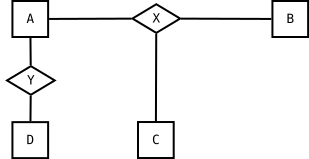
\includegraphics[height=150pt]{resources/er-to-neo4j.pdf}
	\caption{Example conversion of an ER diagram into a \neoj graph}
	
	%Create (a1:A {name: 'A1'}), (b1:B {name: 'B1'}), (b2:B {name: 'B2'}), (c1:C {name: 'C1'}), (c2:C {name: 'C2'}), (d1:D {name: 'D1'}), (d2:D {name: 'D2'}), (x1:X {name: 'X1'}), (x2:X {name: 'X2'}), (a1)-[:XA]->(x1), (x1)-[:XB]->(b1), (x1)-[:XC]->(c1), (a1)-[:Y]->(d1), (a1)-[:Y]->(d2), (a1)-[:XA]->(x2), (x2)-[:XB]->(b2), (x2)-[:XC]->(c2)
	
	\label{fig:example-er-diagram}
\end{figure}

\subsection{\masymos}
\label{sec:background:graph-db:masymos}

This work is mainly based on \masymos, "a graph database for simulation models and associated data" \citep{Henkel2015}, which is implemented using \neoj \citep{Robinson2013}

Since \masymos is developed for "storing and retrieving structural information of biological models" \citep{Henkel2015}, it needs to incorporate mentioned graph representations of simulation networks and an efficient way to query those. Therefore \neoj was the ideal choice, as it works as large property graph, but also "follows fundamental properties of databases, i.e. the ACID principles. \citep{Henkel2015}

The internal schema used by \masymos, as shown in figure \ref{fig:background:graph-db:masymos}, features a \texttt{DOCUMENT} node as standard entry point. This \texttt{DOCUMENT} node represents the actual \xml document and has only one direct child: The \texttt{MODEL} node, which is the entry point for the actual model and represents the \xml root node.

Beyond these two nodes, the schema depends on the format, encoding the imported model. For \sbml the \texttt{MODEL} node is linked to compartments, species, and reactions. Which on the other hand can be linked among each other, expressing relations like reaction reactants and products, or association to a compartment.
Whereby in \cellml the \texttt{MODEL} node links to components, which again contain variables and mathematical expressions, manipulating other variables.

Further semantic annotations, like ontology terms or publication, and author relations, are represented by additional nodes and link to the corresponding ontology term, stored in \neoj, or the interrelated publication or person node. 
Ontology terms are imported according to their hierarchical structure from the \owl representation, which preserves the classification information and therefore allows for searching for abstract terms, but still support traversing to more detailed terms and vice versa.
Commonly imported ontologies are System Biology Ontology\footnote{\url{http://purl.bioontology.org/ontology/SBO}} (SBO), Gene Ontology\footnote{\url{http://purl.bioontology.org/ontology/GO}} (GO), KiSAO\footnote{\url{http://purl.bioontology.org/ontology/KISAO}} and Chebi Ontology\footnote{\url{http://purl.bioontology.org/ontology/CHEBI}}

In addition to explicit links, the graph database back-end of \masymos allows to include implicit links into analysis (those with more than one hop in the graph). Implicit links can link between two models, published by the same person or between model with, common annotations, or even between models using annotations of the same ontology branch.
Further, to allow easy upwards traversal, all relations also feature a common relation to the next higher node in hierarchy, called \texttt{belongs\_to}.

\todo{paragraph about shortcomings}
\begin{figure}[h]
	\centering
	\includegraphics[width=\textwidth]{resources/masymos_struc_figure2.eps}
	\caption{Structure representing \sbml and \cellml models in \masymos. Figure taken from \citealt{Henkel2015}.}
	\label{fig:background:graph-db:masymos}
\end{figure}

\begin{comment}
% following some quotes from the Henkel2015 paper
\begin{itemize}
	\item This work is based on MaSyMoS, "a graph database for simulation models and associated data" \citep{Henkel2015}
	\subitem \citep{Henkel2015} Many models in public databases encode networks that can be represented as graphs
	\subitem \citep{Henkel2015} relational databases were developed for homogeneous, structured data, e.g. numerical data
	\subitem \citep{Henkel2015} Designing a relational representation for these links and keeping the database efficient at the same time are impossible
	
	\item \citep{Henkel2015} MaSyMos is a database based on neo4j for storing and retrieving structural information of biological models
	\subitem \citep{Henkel2015} We chose the graph database Neo4J (25)
	\subitem \citep{Henkel2015} follows the fundamental properties of databases, i.e. the ACID principles
	
	\item \citep{Henkel2015} biological models are represented in heterogenous data structures e.g. networks. Traditional relational databases are build to quickly process highly structured data in tables, therefore they are less efficient in storing and retrieving standard encoded models, due to their highly linked structure
	\subitem \citep{Henkel2015} No unified schema exists for models and meta-data, making it difficult to define a relational database schema
	\subitem \citep{Henkel2015} highly linked models, model entities and meta-data are difficult to represent in a table-based relational database
	\item \masymos data model and structure
	\subitem \citep{Henkel2015} document root node is created for each data item
	\subitem each model is represented by a model node
	\subsubitem entry point for each model import is a document node
	\subitem \citep{Henkel2015} Attached to the model node are annotation nodes, including the reference publication
	\subitem in SBML compartments, species and reactions are linked to the model node
	\subitem in CellML each component is linked to the model node, further containing variables and mathematical relationships to manipulate other variables
	\subsubitem \citep{Henkel2015} component contains vari- ables and mathematical relationships that manipulate those variables
	\subitem Experiment setups are stored under a SEDML node, instead of a model node. In comparison to species, reactions, compartments or components the SEDML node has links to Modelreference nodes, as well as nodes pointing to different model entities used in plots. Nevertheless no processing information is stored in the database.
	\subsubitem \citep{Henkel2015} SEDML node serves as the anchor for an experiment
	\subsubitem \citep{Henkel2015} Modelreference node links the experiment to all Model nodes used in the simulation
	\subsubitem \citep{Henkel2015} do not store the specific processing of a model entity
	\subitem Semantic annotations and cross-references from the models are stored as seperate nodes and linked to the ontology node representing the used ontology term.
	\subsubitem \citep{Henkel2015} Semantic annotations and cross-references
	\subsubitem \citep{Henkel2015} We parse these ontologies and add all concepts and relations as nodes and edges, respectively.
	\subitem ensure an easy traversal upwards, a connection is created from each node of the stored model that points to the parent of the current node. The corresponding edges are named belongsTo]
	\item Linking model related data
	\subitem main advantage to prior mentioned storage in relational databases is the possibility to flexibly link data between different domains. //Henkel et al.// describes 3 different links, which are currently implemented: 1. links between (model) annotations and the corresponding ontology term 2. links between models or model entities and SEDML simulation descriptions or respectively SEDML variables 3. links between model entities in different standard format representation
	\subsubitem \citep{Henkel2015} The main advantage of the previously described concept is its possibility to define flexible links between the data do\item mains)
	\subsubitem \citep{Henkel2015} links between annotations (in SBML, CellML and SED-ML) and ontology concepts)
	\subsubitem \citep{Henkel2015} links between models (in SBML or CellML format) and SED-ML
	\subsubitem \citep{Henkel2015} link is that between a model and a simulation description
	\subsubitem \citep{Henkel2015} links between model entities and SED-ML variables
	\subsubitem \citep{Henkel2015} links between model entities from different model rep- resentation formats
	\subitem \citep{Henkel2015} For each annotation in a model we add an explicit link to the data entry in the ref- erenced bio-ontology
	\subitem This link is shared between all models using this annotation, regardless of the format
	\subitem Further to explicit links (one hop in the graph), MaSyMoS is able to determine implicit links between different models. Those can be established over shared resources like a publication, publication author or annotations with common bio-ontologies. Regarding a publications the database may establish connections based on the likelihood of names by Hemming Distance, resulting in a confidence which can be increased, "" if the entities' annotations match
	\subsubitem \citep{Henkel2015} In addition, we determine implicit links between models of different representation formats
	\subsubitem \citep{Henkel2015} If two models share a publication, the systems can infer implicit links between those entities that are equally named
	\item Implementation
	\subitem MaSyMoS is designed to run as both standalone commandline application with embedded neo4j and as an extension to the neo4j server. Latter is controlled by an unmanaged neo4j plugin providing a RESTful json interface.
	\subitem Same interface also cooperates with the retrieval engine Morre, by providing endpoints to query different search indexes.
	
	\item MaSyMoS project structure
	\subitem The MaSyMoS project is divided into 3 different modules: MaSyMoS-core, Morre and a CLI.
	\subitem The core module contains the logic of the database and communicates directly with neo4j. It consists of routines and a Java API to import models, experiments and ontologies. Further it fetches linked information from common bio-ontologies and manages, updates and queries Lucene indexes.
	\subitem The Command Line Interface (CLI) provides a user interface, to easily interact with the API provided by the core module. It's main purpose was to simplify the development process by skipping the deployment step. Instead it is possible to directly interact with and debug MaSyMoS
	\subitem The Morre module is similiar to the CLI, by providing an way to interact with the core. But instead of providing a user interface, Morre is loaded as neo4j unmanaged extension and exposes a RESTful interface, which can be used to query the Lucene indexes or to push and update models to the database.
\end{itemize}
\end{comment}
\todo{Pictures}

